% ==============================================================================
%
%                             Appendices
%
% ==============================================================================
\chapter{Appendices}\label{chp:appendices}

\section{Aufgabenstellung 2018 P6 Distributed FPGA} \label{app:aufgabenstellung}
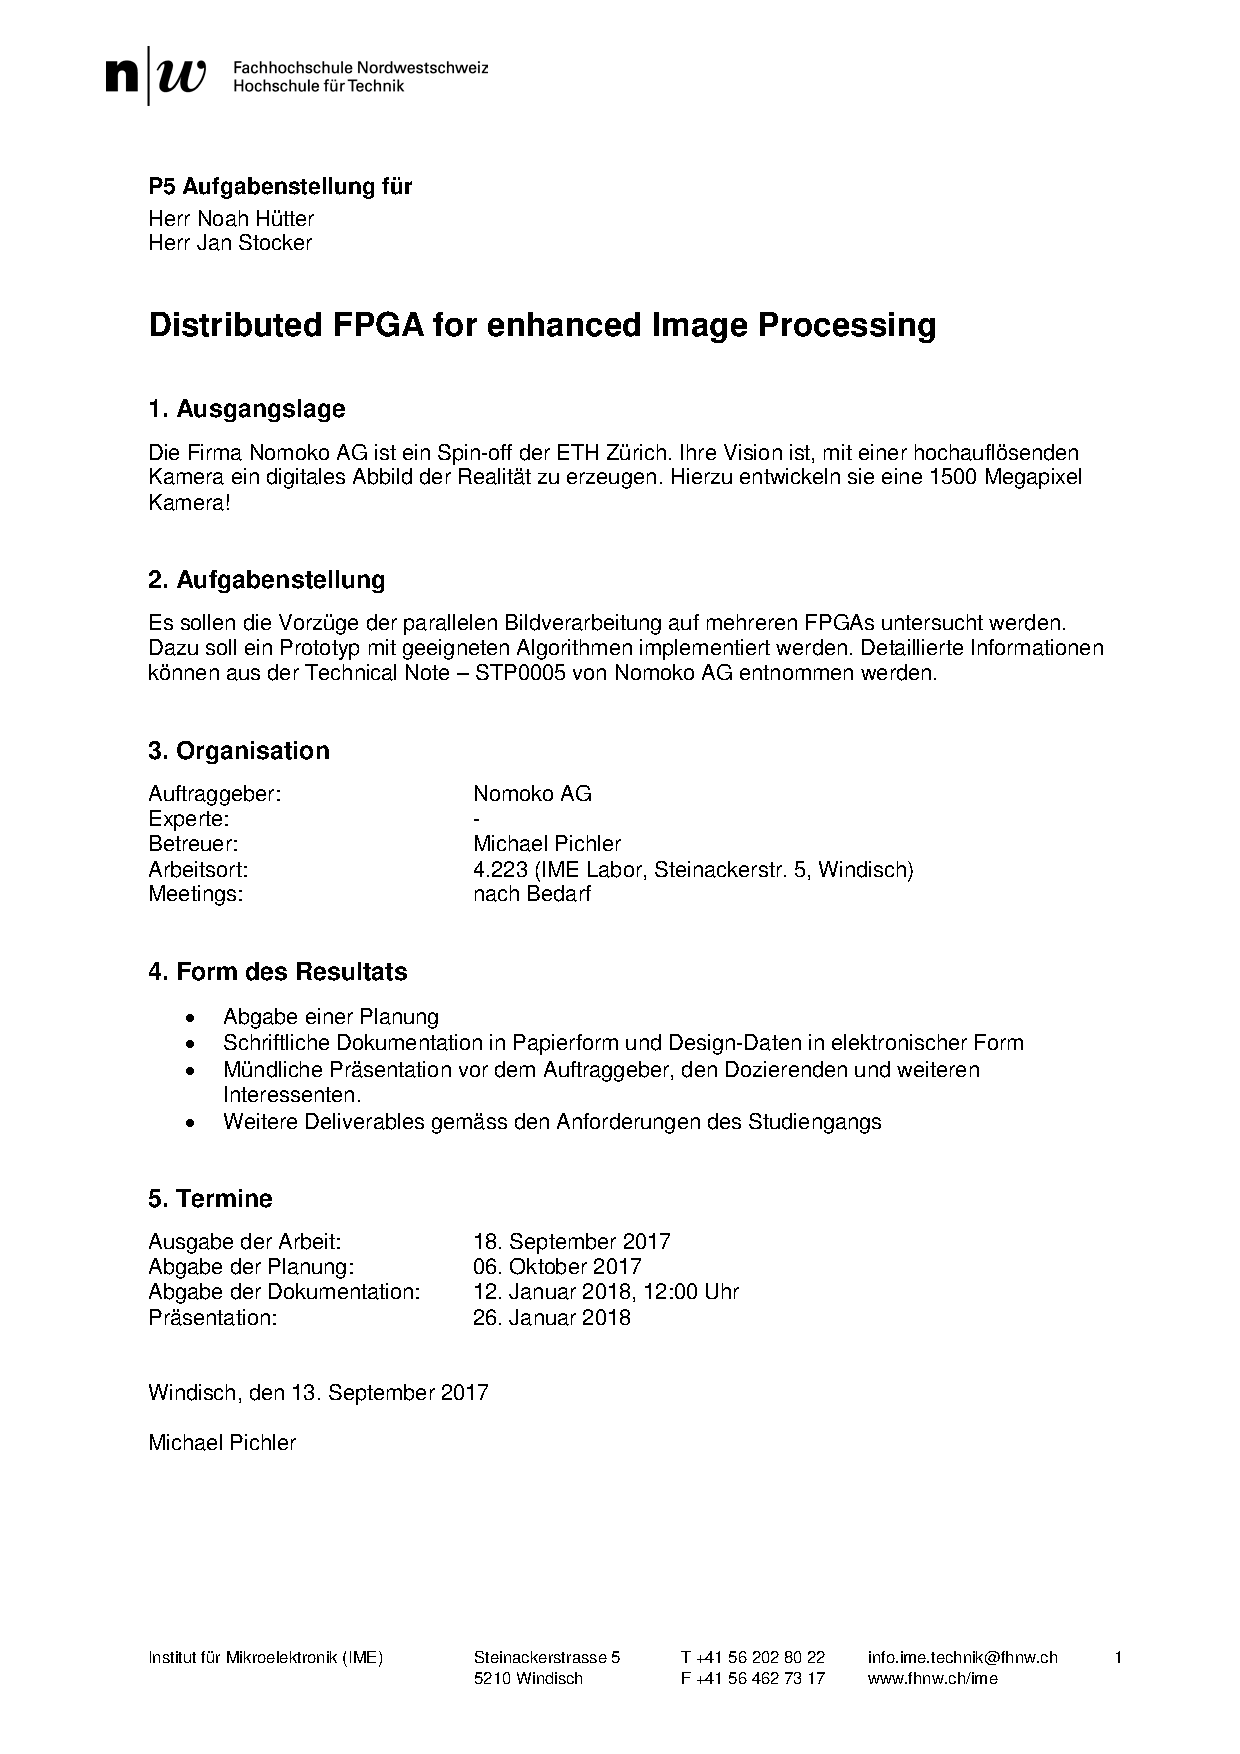
\includepdf[pages=-,scale=1,linktodoc=false]{appendices/Aufgabenstellung_2017_P5_Distributed_FPGA_comb.pdf}

\section{Technicial requirements} \label{app:technicial_requirements}
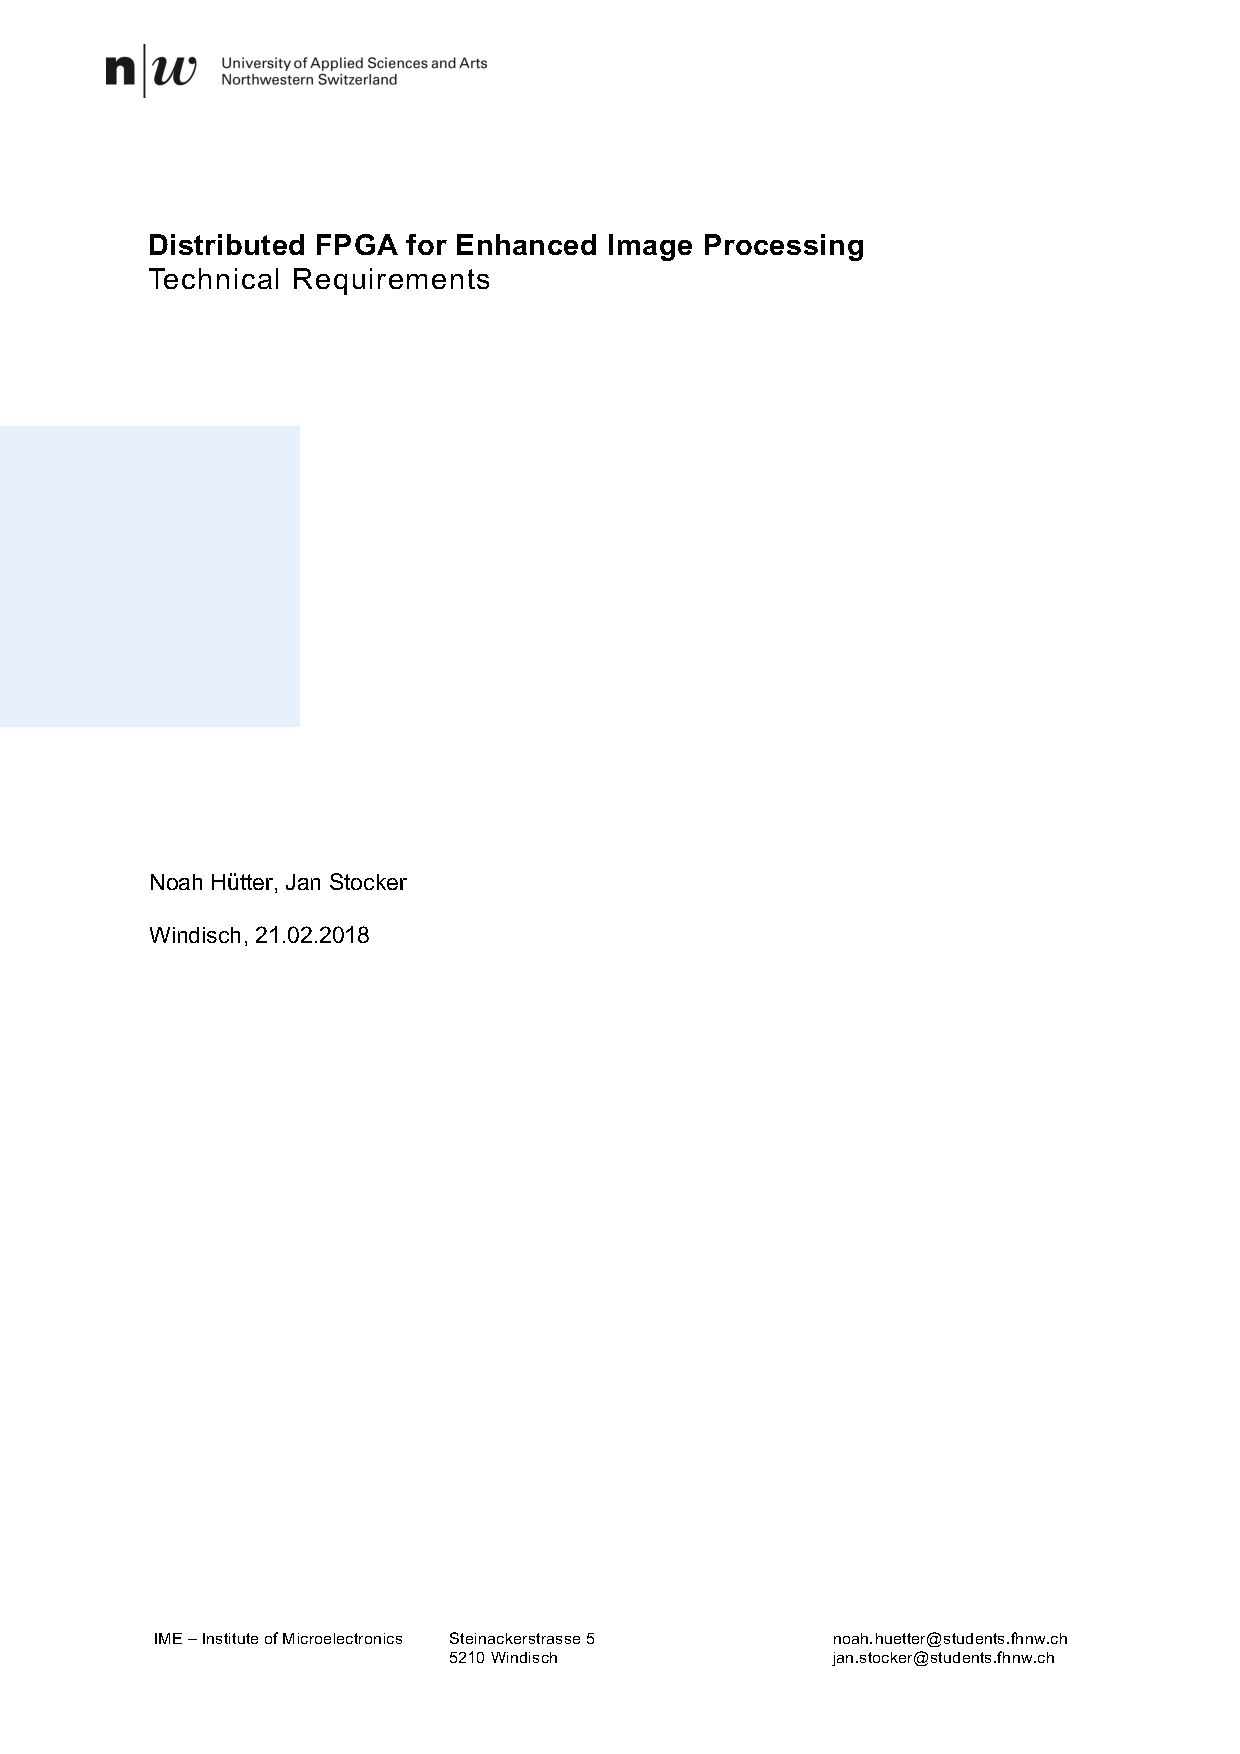
\includepdf[pages=-,scale=1,linktodoc=false]{appendices/technical_requirements_P6.pdf}

\section{Data types of the Wallis filter} \label{app:datatypes}
\begin{table}[H]
    \centering
    \begin{tabularx}{\textwidth}{l l}
        \toprule
        Name & Description \\
        \midrule
        iPxl & 			Pixel from the input image which is calculated \\
        g\_Mean &  		Global mean of the output image \\
        g\_Var &  		Global variance of the output image \\
        n\_Mean &		Mean of the neighborhood \\
        n\_Var &  		Variance of the neighborhood \\
        brightness & 	Brightness factor \\
        contrast & 		Contrast factor \\
        b\_gMean &  	Multiplication of brightness and global mean\\
        ci\_gVar &  	Multiplication of (1 - contrast) and global variance\\
        tmp\_Num &  	Temporary numerator of the division without contrast\\
        num &   		Numerator of the division with contrast\\
        c\_nVar &  		Multiplication of contrast and neighborhood variance\\
        bi\_nMean &  	Multiplication of (1 - brigthness) and neighborhood mean\\
        den\_Var & 		Denumerator of the division \\
        rec & 			Variable has value 1 to calculate a reciprocal division\\
        den & 			Result of the reciprocal division\\
        div &  			Result of the entire Wallis filter division\\
        w\_pixel &  	Output pixel from the Wallis filter\\
        \bottomrule
    \end{tabularx}
    \caption{Description of data types in the Wallis filter division}
\end{table}

\clearpage

\section{UDP File Transfer} \label{app:uftspec}

\includepdf[pages=-,scale=1,linktodoc=false]{appendices/UDP_File_Transfer.pdf}

\section{UDP file transfer calculation} \label{app:uftcalc}
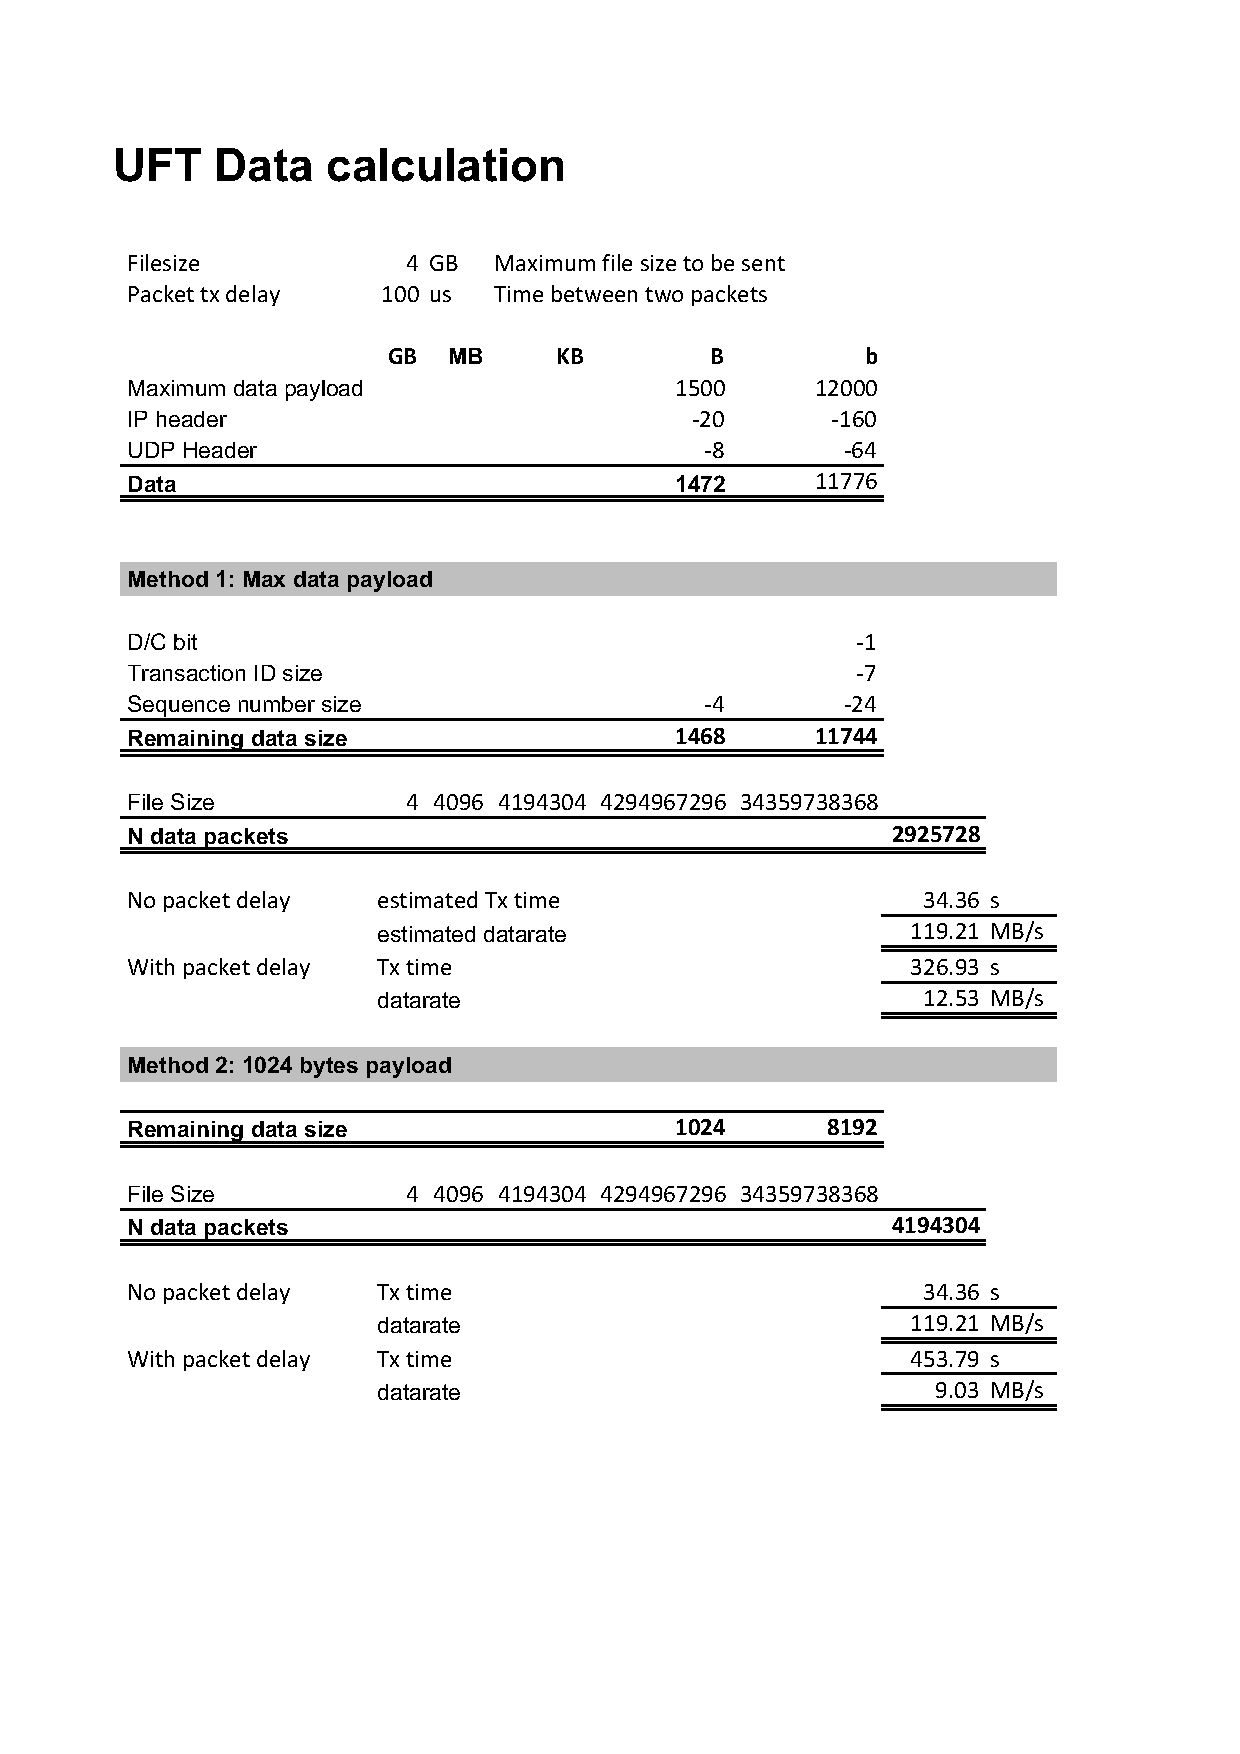
\includepdf[pages=-,scale=1,linktodoc=false]{appendices/uftcalc.pdf}

\section{Images for Wallis filter} \label{app:images_wallis}
\begin{figure}[H]
    \centering
    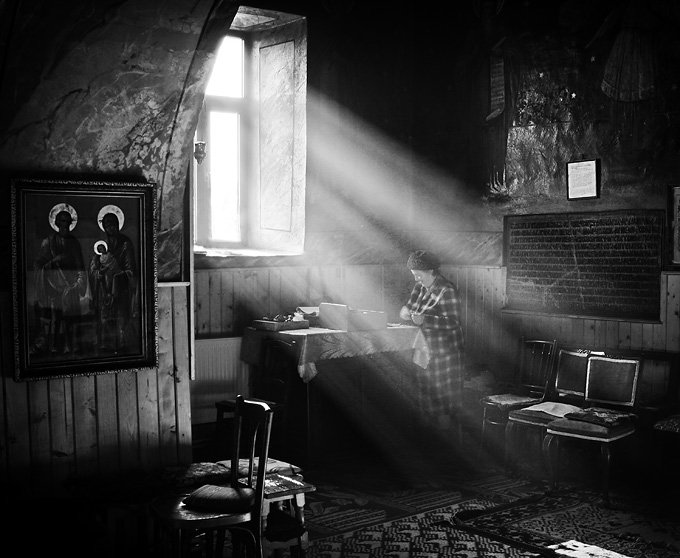
\includegraphics[width=0.8\textwidth]{appendices/ref_room.png}
    \caption{Source image room for the image processing verification}
    \label{fig:ref_room}
\end{figure}

\begin{figure}[H]
    \centering
    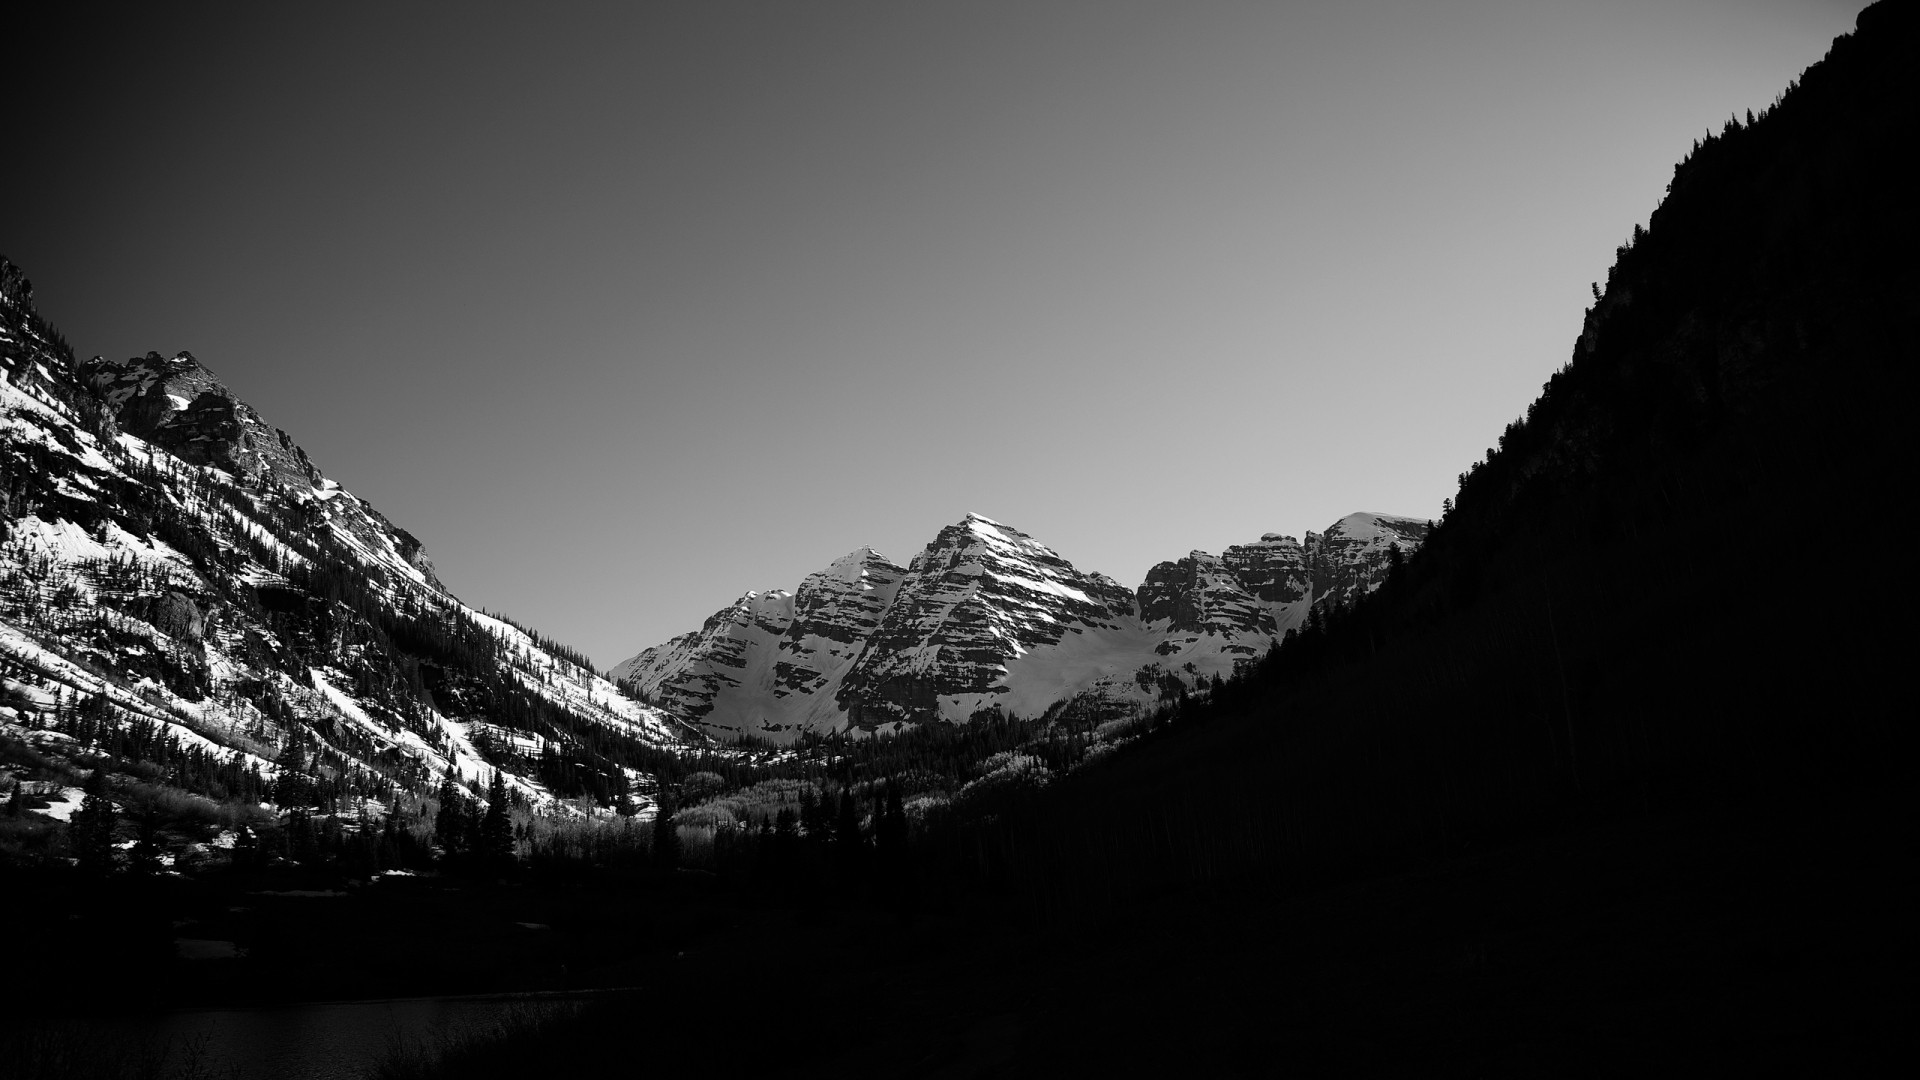
\includegraphics[width=0.8\textwidth]{appendices/ref_mountain.png}
    \caption{Source image mountain for the image processing verification}
    \label{fig:ref_mountain}
\end{figure}

\section{Derivations} \label{app:derivations}
\subsection{Theoretical maximum throughput of VHDL solution} \label{app:derivations:theomax}

\begin{align}
    b  & = \frac{i_p}{t_t} \\
       & = \frac{i_w i_h}{t_i+(i_h-w_l+1)t_r} \\
       & = \frac{i_w i_h}{(\frac{i_w}{b_e}+d_l)w_l+(i_h-w_l+1)(\frac{i_w}
       {b_e}+d_l)} \\
       & = \frac{i_w i_h}{(\frac{i_w}{b_e}+d_l)(i_h+1)} \\
       & = \frac{i_w i_h}{d_l(i_h+1)+\frac{i_w}{b_e}(i_h+1)} \\
       & \approx \frac{i_w}{d_l+\frac{i_w}{b_e}}
    \label{eq:theomaxb}
\end{align}
\begin{tabular}{rl}
    $b     =$ & theoretical throughput of VHDL solution \\
    $i_p   =$ & total image pixels \\
    $t_t   =$ & total processing time \\
    $i_w   =$ & image width \\
    $i_h   =$ & image height \\
    $t_i   =$ & time to send the initial lines \\
    $w_l   =$ & windows length \\
    $t_r   =$ & iterration time to process one line \\
    $b_e   =$ & ethernet throughput \\
    $d_l   =$ & delay between sending two image lines \\
\end{tabular} \\

\subsection{Theoretical maximum throughput of VHDL Wallis core} 
\label{app:derivations:theomaxvhdlwallis}

\begin{align}
    b  & = \frac{i_p}{t_w} &\\
       & = \frac{i_wi_h}{\frac{n_{ps}}{b_w}} &\\
       & = \frac{i_w i_h b_w}{w_l i_w (i_h-w_l+1)} &\\
       & = \frac{i_hb_w}{w_l (i_h-w_l+1)} &\\
       & = \frac{b_w}{w_l (1-\frac{w_l}{i_h}+\frac{1}{i_h})} &\\
       & \approx \frac{b_w}{w_l} &(i_h \to \infty)
    \label{eq:theomaxvhdlwallis}
\end{align}
\begin{tabular}{rl}
    $b     =$ & theoretical throughput of VHDL Wallis filter \\
    $i_p   =$ & total image pixels \\
    $t_w   =$ & total processing time of Wallis filter \\
    $i_w   =$ & image width \\
    $i_h   =$ & image height \\
    $n_{ps}=$ & Number of pixels processed by Wallis filter on input \\
    $b_w   =$ & throughput of Wallis filter \\
    $w_l   =$ & window length \\
\end{tabular} \\
